\documentclass[sigconf]{acmart}

%% --- ACM METADATA ---------------------------------------------------
%% NOTE: Update these fields with actual conference details before submission
\copyrightyear{2025}
\acmYear{2025}
\setcopyright{rightsretained}
%% Uncomment and update with real conference details:
% \acmConference[CONF'25]{Conference Name}{Month Year}{City, Country}
% \acmBooktitle{Conference Name, Month Year, City, Country}

%% For preprint/draft mode, use these settings:
\settopmatter{printacmref=false}
\renewcommand\footnotetextcopyrightpermission[1]{}

%% --- PACKAGES -------------------------------------------------------
\usepackage{tikz}
\usetikzlibrary{automata, positioning, arrows.meta, bending, shapes}
\usepackage{algorithm}
\usepackage[noend]{algpseudocode}
\usepackage{amsmath}
\usepackage{amssymb}
\usepackage{listings}
\usepackage{xcolor}
\usepackage{booktabs}
\usepackage{multirow}

%% --- THEOREM ENVIRONMENTS ------------------------------------------
\theoremstyle{plain}
\newtheorem{theorem}{Theorem}
\newtheorem{lemma}[theorem]{Lemma}
\newtheorem{corollary}[theorem]{Corollary}
\newtheorem{proposition}[theorem]{Proposition}

\theoremstyle{definition}
\newtheorem{definition}{Definition}

%% --- CODE LISTING STYLE ---------------------------------------------
\definecolor{codegreen}{rgb}{0,0.6,0}
\definecolor{codegray}{rgb}{0.5,0.5,0.5}
\definecolor{codepurple}{rgb}{0.58,0,0.82}
\definecolor{backcolour}{rgb}{0.95,0.95,0.92}

\lstdefinestyle{mystyle}{
    backgroundcolor=\color{backcolour},
    commentstyle=\color{codegreen},
    keywordstyle=\color{magenta},
    numberstyle=\tiny\color{codegray},
    stringstyle=\color{codepurple},
    basicstyle=\ttfamily\footnotesize,
    breakatwhitespace=false,
    breaklines=true,
    captionpos=b,
    keepspaces=true,
    numbers=left,
    numbersep=5pt,
    showspaces=false,
    showstringspaces=false,
    showtabs=false,
    tabsize=2
}
\lstset{style=mystyle}

%% --- TITLE & AUTHORS ------------------------------------------------
\title[Scanpath Pattern Recognition in ECG Interpretation]{Scanpath Pattern Recognition in ECG Interpretation using Probabilistic Finite Automata: A Formal Language Approach to Visual Expertise}

\author{Gougasse Hamza, Abderrahmane Fouzi Abouzaid}
\affiliation{%
  \institution{Mohammed VI Polytechnic University}
  \city{Rabat}
  \country{Morocco}
}
\email{hamza.gougasse@um6p.ma - abderrahmane.abouzaid@um6p.ma}

%% --- CCS CONCEPTS & KEYWORDS ----------------------------------------
\begin{CCSXML}
<ccs2012>
  <concept>
    <concept_id>10003120.10003121.10003124.10010866</concept_id>
    <concept_desc>Human-centered computing~Eye tracking</concept_desc>
    <concept_significance>500</concept_significance>
  </concept>
  <concept>
    <concept_id>10010405.10010444.10010449</concept_id>
    <concept_desc>Applied computing~Health informatics</concept_desc>
    <concept_significance>300</concept_significance>
  </concept>
  <concept>
    <concept_id>10003752.10003790.10003792</concept_id>
    <concept_desc>Theory of computation~Automata over probabilistic words</concept_desc>
    <concept_significance>300</concept_significance>
  </concept>
</ccs2012>
\end{CCSXML}

\ccsdesc[500]{Human-centered computing~Eye tracking}
\ccsdesc[300]{Applied computing~Health informatics}
\ccsdesc[300]{Theory of computation~Automata over probabilistic words}

\keywords{Probabilistic Finite Automata, ECG Interpretation, Eye Tracking, Formal Languages, Grammatical Inference, Stochastic Regular Languages}

%% --- DOCUMENT START -------------------------------------------------
\begin{document}

%% --- ABSTRACT -------------------------------------------------------
\begin{abstract}
The 12-lead electrocardiogram (ECG) is a critical diagnostic tool, yet novice practitioners still misinterpret 36,50\% of cases due to unstructured visual search strategies.
Whereas expert interpretation relies on rapid, hypothesis-driven pattern recognition and systematic regional coverage, novices display scattered and incomplete search behaviour.
This paper introduces a formal-language framework for modelling visual expertise using probabilistic automata.
We model stochastic sequences of eye fixations with probabilistic finite automata (PFA).
Using the PhysioNet Eye Tracking Dataset ($N=63$), we apply a Grid Overlay Method to discretise gaze fixations into a semantic spatio-temporal alphabet $\Sigma$ of 22 symbols.
We define expert and novice scanpaths as stochastic regular languages and instantiate this framework with two PFAs trained on consultant/fellow versus medical-student scanpaths.
We present two classifiers: (1)~a baseline PFA log-likelihood-ratio classifier, and (2)~an improved pipeline combining PFA-derived transition features with rich AOI-level numeric features (fixation counts, temporal allocation, revisit patterns) and a Random Forest classifier.
In a participant-level leave-one-out cross-validation on 35 clinicians (19~expert, 16~novice; 350~scanpaths total), the improved classifier achieves 94.3\% accuracy (Precision: 0.95, Recall: 0.95, F1: 0.95, AUC-ROC: 0.95).
We formally show that scanpath likelihoods can be evaluated in $O(n)$ time for fixed-size PFAs, and we interpret the log-likelihood-ratio decision rule as an instance of the Neyman,Pearson lemma.
This work bridges cognitive psychology and formal language theory, providing mathematically grounded building blocks for interpretable, automata-based intelligent tutoring systems.
\end{abstract}

\maketitle

% ==========================================
% 1. INTRODUCTION
% ==========================================
\section{Introduction}

\subsection{The Clinical Problem}
Electrocardiography remains the primary non-invasive diagnostic tool for cardiac pathology, with over 300 million ECGs recorded annually worldwide~\cite{davies2012}.
Despite its ubiquity, accurate interpretation remains challenging.
The literature consistently documents a ``competence gap,'' where non-specialist accuracy ranges from 36,50\%~\cite{wood2013}.
This performance divergence stems less from declarative knowledge deficits than from procedural strategy differences:
experts employ rapid, hypothesis-driven ``System~1'' pattern recognition characterised by systematic regional examination (inferior $\rightarrow$ lateral $\rightarrow$ anterior leads), whereas novices exhibit ``scattergun'' behaviour and fail to complete critical verification loops~\cite{bond2018}.

\subsection{The Gap in Current Analysis}
To investigate these strategies, researchers increasingly employ eye-tracking.
However, the standard analytical toolkit, heatmaps, fixation-duration statistics, and global metrics such as ``time to first fixation'', is fundamentally limited~\cite{sqalli2022}.
These approaches aggregate spatial data while largely obliterating the temporal dimension that is crucial for understanding diagnostic reasoning.
For example, a heatmap reveals \emph{that} a clinician examined Lead~II and Lead~V1, but not \emph{whether} they were examined in the clinically meaningful order (rhythm assessment $\rightarrow$ morphology verification).
Most existing analyses thus fail to capture the \emph{grammar} of visual scanpaths, the underlying structural rules governing expert sequential behaviour.

\subsection{Proposed Formal Solution}
We posit that expert ECG interrogation is not a random walk but a structured formal language: a ``visual sentence'' composed of anatomical ``phonemes.''
We hypothesise that the set of valid expert scanpaths forms a \emph{stochastic regular language} $\mathcal{L}_{\text{exp}} \subseteq \Sigma^*$.
Consequently, the cognitive strategy can be modelled by probabilistic finite automata (PFA).
A PFA extends a deterministic finite automaton (DFA) by assigning probability distributions to state transitions, capturing both canonical expert paths and the stochastic variability of human behaviour~\cite{vidal2005}.
This formalism enables us to:
(1) generate synthetic expert scanpaths,
(2) compute likelihood-based scores for classification, and
(3) provide interpretable, state-based feedback on deviations from expert behaviour.

\subsection{Contributions}
This paper makes the following contributions:
\begin{enumerate}
    \item A formal definition of ECG scanpaths as strings generated by a 5-tuple PFA, together with a semantics in terms of stochastic regular languages.
    \item The Grid Overlay Method for discretising continuous gaze coordinates into a semantic alphabet with temporal encoding of short versus long fixations.
    \item A PFA-based baseline classifier that trains separate expert and novice automata and uses a normalised log-likelihood ratio as a decision score.
    \item An improved classifier that augments PFA-derived transition features with AOI-level numeric features (fixation variability, temporal allocation, revisit patterns) and applies feature selection with a Random Forest.
    \item Rigorous proofs establishing regularity of the induced scanpath languages and $O(n)$ complexity for likelihood computation in fixed-size PFAs.
    \item An empirical evaluation on the PhysioNet eye-tracking dataset achieving 94.3\% participant-level accuracy, 0.95 precision, 0.95 recall, 0.95 F1-score and 0.95 AUC-ROC under leave-one-out cross-validation.
\end{enumerate}

% ==========================================
% 2. RELATED WORK
% ==========================================
\section{Related Work}

\subsection{Visual Expertise in Medical Imaging}
The ``global,local'' search model established by Kundel et al.~\cite{kundel1978} suggests that experts rapidly scan for a gestalt impression before focusing on diagnostic details.
In cardiology, Bond et al.~\cite{bond2018} employed Levenshtein edit distance to compare scanpaths and found that higher diagnostic error rates correlate with increased scanpath entropy.
Davies et al.~\cite{davies2012} demonstrated that expert scanpaths exhibit significantly lower variability and more structured regional coverage.
These string-edit approaches, however, provide similarity metrics without generative models of the underlying cognitive process:
they quantify \emph{how different} scanpaths are without explaining \emph{why}.

\subsection{Scanpath Sequence Analysis}
Outside medicine, sequence-mining techniques have been applied to web navigation, reading comprehension, and visual search.
Eraslan et al.~\cite{eraslan2019} comprehensively reviewed scanpath analysis methods and highlighted the limitations of vector-based metrics for tasks with rich semantics.
Most existing methods rely on pairwise alignment algorithms (Needleman,Wunsch, Smith,Waterman), which scale quadratically $O(N^2)$ and cannot capture branching logic, the loops and conditionals inherent in hypothesis-driven clinical reasoning.
Hidden Markov Models (HMMs) have been applied to eye-tracking~\cite{dupont2005}, but their hidden states are often hard to interpret compared to explicit automaton states.

\subsection{Grammatical Inference for Behavioural Modelling}
Grammatical inference (GI) learns formal languages from example strings.
The Alergia algorithm~\cite{carrasco1994} and Red,Blue state-merging framework~\cite{verwer2014} are standard approaches for learning stochastic regular languages.
They have been widely applied in software verification and protocol reverse engineering~\cite{muskardin2021}, but their use for modelling biological human behaviour remains limited.
Our work offers a synthesis of grammatical inference and medical cognitive modelling, providing interpretable, state-based explanations of expert reasoning.

% ==========================================
% 3. FORMAL MODEL
% ==========================================
\section{Formal Model}

In this section we give the mathematical framework for modelling ECG interpretation scanpaths as stochastic regular languages.

\subsection{Preliminaries and Notation}

\begin{definition}[Alphabet]
Let $\Sigma$ be a finite, non-empty set called the \emph{alphabet}.
Elements $\sigma \in \Sigma$ are called \emph{symbols}.
\end{definition}

\begin{definition}[String and Language]
A \emph{string} $w = \sigma_1\sigma_2\ldots\sigma_n$ is a finite sequence of symbols from $\Sigma$.
The set of all strings over $\Sigma$ is denoted $\Sigma^*$ and includes the empty string $\varepsilon$.
A \emph{language} $L \subseteq \Sigma^*$ is a set of strings.
\end{definition}

\begin{definition}[Stochastic Language]
A \emph{stochastic language} over $\Sigma$ is a probability distribution $P: \Sigma^* \rightarrow [0,1]$ such that $\sum_{w \in \Sigma^*} P(w) = 1$.
\end{definition}

\subsection{Alphabet Design}

We design the ECG scanpath alphabet to capture both spatial location and cognitive processing depth.
Let
\[
\mathcal{R} = \{I, II, III, aVR, aVL, aVF, V1, V2, V3, V4, V5, V6, Rh\}
\]
denote the 12 standard ECG leads plus the rhythm strip region.

\begin{definition}[ECG Scanpath Alphabet]
The alphabet $\Sigma$ is
\begin{equation}
\Sigma = \{ L_s, L_l \mid L \in \mathcal{R} \},
\end{equation}
where the subscript $s$ denotes a \emph{short} fixation ($<200$\,ms, scanning behaviour) and $l$ denotes a \emph{long} fixation ($\geq 200$\,ms, cognitive processing).
In the full 12-lead set this gives $|\Sigma| = 26$; in practice, leads I and III are not annotated as separate AOIs in our dataset, yielding $|\Sigma| = 22$.
\end{definition}

The 200\,ms threshold is well-established in cognitive psychology as distinguishing perceptual scanning from active information processing~\cite{kundel1978}.

\begin{definition}[Scanpath]
A \emph{scanpath} is a string $w = \sigma_1\sigma_2\ldots\sigma_n \in \Sigma^*$ representing the temporal sequence of fixation events during ECG interpretation.
\end{definition}

\textbf{Example.}
The string
\[
w = Rh_l \cdot II_l \cdot V1_s \cdot V2_s \cdot II_l \cdot I_l
\]
represents a scanpath where the clinician:
(1) examines the rhythm strip (long),
(2) studies Lead~II for P-waves (long),
(3) scans V1,V2 (short),
(4) returns to Lead~II for verification (long), and
(5) examines Lead~I (long).

\subsection{Expert and Novice Stochastic Languages}

\begin{definition}[Expert and Novice Scanpath Languages]
Let $\mathcal{L}_{\text{exp}}, \mathcal{L}_{\text{nov}} \subseteq \Sigma^*$ denote the \emph{expert} and \emph{novice} scanpath languages: the sets of scanpath strings consistent with systematic consultant/fellow ECG interpretation and with first-/second-year medical students, respectively.
Each language is associated with a stochastic distribution $P_{\text{exp}}$ or $P_{\text{nov}}$ over $\Sigma^*$.
\end{definition}

\subsection{Probabilistic Finite Automata}

\begin{definition}[Probabilistic Finite Automaton]
A \emph{probabilistic finite automaton} (PFA) is a 5-tuple $M = (Q, \Sigma, \delta, \pi, F)$ where:
\begin{itemize}
    \item $Q$ is a finite set of states;
    \item $\Sigma$ is the input alphabet;
    \item $\delta: Q \times \Sigma \times Q \rightarrow [0,1]$ is the transition probability function satisfying
    \begin{equation}
    \forall q \in Q: \sum_{\sigma \in \Sigma} \sum_{q' \in Q} \delta(q, \sigma, q') + \gamma(q) = 1,
    \end{equation}
    where $\gamma(q)$ is the termination probability at state $q$;
    \item $\pi: Q \rightarrow [0,1]$ is the initial state distribution with $\sum_{q \in Q} \pi(q) = 1$;
    \item $F \subseteq Q$ is the set of accepting states.
\end{itemize}
\end{definition}

For conceptual analysis we consider a high-level PFA in which states correspond to clinically meaningful phases of interpretation (rhythm assessment, inferior leads, lateral leads, anterior leads, verification).
In the concrete implementation used for our experiments (Section~\ref{sec:methodology}), we learn PFAs from data using the Alergia state-merging algorithm~\cite{carrasco1994}, which automatically determines the number of states (23 states for both expert and novice PFAs in our experiment).

\begin{figure}[t]
    \centering
    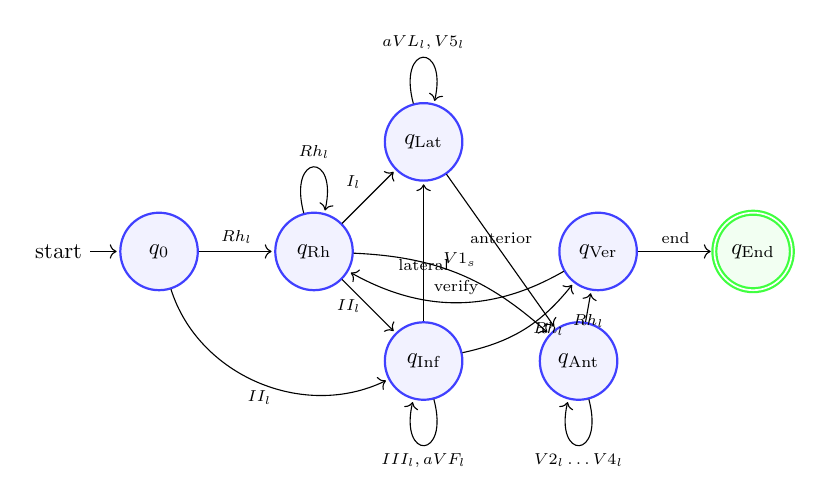
\begin{tikzpicture}[shorten >=1pt, node distance=2.4cm, on grid, auto,
        scale=0.82, transform shape,
        state/.style={circle, thick, draw=blue!75, fill=blue!5, minimum size=12mm},
        accepting/.style={double, draw=green!75, fill=green!5}]
        
        % Nodes
        \node[state, initial] (q0) {$q_0$};
        \node[state] (qRh) [right=of q0] {$q_{\text{Rh}}$};
        \node[state] (qInf) [below right=of qRh] {$q_{\text{Inf}}$};
        \node[state] (qLat) [above right=of qRh] {$q_{\text{Lat}}$};
        \node[state] (qAnt) [right=of qInf] {$q_{\text{Ant}}$};
        \node[state] (qVer) [right=of qRh, xshift=2cm] {$q_{\text{Ver}}$};
        \node[state, accepting] (qEnd) [right=of qVer] {$q_{\text{End}}$};

        % Transitions
        \path[->]
            (q0) edge node {\scriptsize $Rh_l$} (qRh)
            (q0) edge [bend right=50] node [below] {\scriptsize $II_l$} (qInf)
            (qRh) edge [loop above] node {\scriptsize $Rh_l$} (qRh)
            (qRh) edge node [left] {\scriptsize $II_l$} (qInf)
            (qRh) edge node [above left] {\scriptsize $I_l$} (qLat)
            (qRh) edge [bend left=20] node [above] {\scriptsize $V1_s$} (qAnt)
            (qInf) edge [loop below] node {\scriptsize $III_l, aVF_l$} (qInf)
            (qInf) edge node [below] {\scriptsize lateral} (qLat)
            (qInf) edge [bend right=20] node [right] {\scriptsize $Rh_l$} (qVer)
            (qLat) edge [loop above] node {\scriptsize $aVL_l, V5_l$} (qLat)
            (qLat) edge node [above] {\scriptsize anterior} (qAnt)
            (qAnt) edge [loop below] node {\scriptsize $V2_l \ldots V4_l$} (qAnt)
            (qAnt) edge node [below] {\scriptsize $Rh_l$} (qVer)
            (qVer) edge [bend left=30] node [above] {\scriptsize verify} (qRh)
            (qVer) edge node {\scriptsize end} (qEnd);
    \end{tikzpicture}
    \caption{Schematic state-transition diagram of a high-level expert PFA $M_{\text{exp}}$.
    The central ``Rhythm Anchor'' structure ($q_{\text{Rh}} \leftrightarrow q_{\text{Ver}}$) represents the hypothesis,verification cycle characteristic of expert reasoning.
    Edge labels are illustrative; our concrete implementation uses symbol-level PFAs with one state per alphabet symbol.}
    \label{fig:pfa}
\end{figure}

\subsection{Formal Properties}

\begin{lemma}[Closure under State Merging]
\label{lem:closure}
Let $M = (Q, \Sigma, \delta, \pi, F)$ be a PFA.
If states $q_i, q_j \in Q$ are merged to form $M' = (Q', \Sigma, \delta', \pi', F')$ with $|Q'| = |Q| - 1$, then $M'$ is also a PFA.
\end{lemma}

\begin{proof}
State merging combines $q_i$ and $q_j$ into a single state $q_{ij}$.
The merged transition function $\delta'$ redistributes probabilities:
\[
\delta'(q, \sigma, q_{ij}) = \delta(q, \sigma, q_i) + \delta(q, \sigma, q_j).
\]
Since the original $\delta$ satisfies the stochasticity constraint
$\sum_{\sigma,q'} \delta(q, \sigma, q') + \gamma(q) = 1$, and merging only combines destination states without altering total probability mass, $\delta'$ also satisfies this constraint.
Because $Q'$ is finite, $M'$ is a valid PFA.
\end{proof}

\begin{theorem}[Regularity of Expert and Novice Languages]
\label{thm:regularity}
If the expert and novice distributions $P_{\text{exp}}$ and $P_{\text{nov}}$ are realised by finite PFAs $M_{\text{exp}}$ and $M_{\text{nov}}$, then $\mathcal{L}_{\text{exp}}$ and $\mathcal{L}_{\text{nov}}$ are stochastic regular languages.
\end{theorem}

\begin{proof}
Learning algorithms such as Alergia~\cite{carrasco1994} construct finite PFAs by starting from a prefix tree acceptor (PTA) built from the training traces and repeatedly merging statistically compatible states.
The PTA is finite with $O(nm)$ nodes for $n$ strings of average length $m$.
By Lemma~\ref{lem:closure}, each merge preserves the PFA structure.
Merging strictly decreases $|Q|$, and the algorithm terminates with $|Q| \geq 1$, so the final structure is a finite automaton.
By Kleene's theorem~\cite{hopcroft2001,sipser2012}, any language recognised by a finite automaton is regular; associating probabilities that sum to~1 yields a stochastic regular language.
The same argument holds for both expert and novice PFAs.
\end{proof}

\begin{algorithm}[t]
  \caption{Scanpath likelihood and perplexity under a PFA}
  \label{alg:likelihood}
  \begin{algorithmic}[1]
    \Require PFA $M = (Q,\Sigma,\delta,\pi,F)$ with termination probabilities $\gamma$, scanpath $w = \sigma_1 \dots \sigma_n$
    \State $\alpha(q) \gets \pi(q)$ for all $q \in Q$ \Comment{initial distribution}
    \For{$i = 1$ to $n$}
      \State $\alpha_{\text{new}}(q) \gets 0$ for all $q \in Q$
      \For{each $q \in Q$}
        \State find successor $q'$ such that $\delta(q,\sigma_i,q') > 0$ (if any)
        \If{such $q'$ exists}
          \State $\alpha_{\text{new}}(q') \gets \alpha_{\text{new}}(q') + \alpha(q) \cdot \delta(q,\sigma_i,q')$
        \EndIf
      \EndFor
      \State $\alpha \gets \alpha_{\text{new}}$
    \EndFor
    \State $P(w) \gets \sum_{q \in Q} \alpha(q)\,\gamma(q)$
    \State $PP(w) \gets P(w)^{-1/n}$ \Comment{perplexity}
    \State \Return $P(w), PP(w)$
  \end{algorithmic}
\end{algorithm}

\begin{theorem}[Recognition Complexity]
\label{thm:complexity}
Given a PFA $M$ with $|Q| = k$ states and a scanpath $w$ of length $n$, the likelihood $P(w \mid M)$ can be computed in $O(n)$ time and $O(k)$ space under the assumption of deterministic emissions (each state,symbol pair leads to at most one successor state).
\end{theorem}

\begin{proof}
Algorithm~\ref{alg:likelihood} maintains a probability vector $\alpha \in \mathbb{R}^k$ where $\alpha(q)$ is the probability of being in state $q$ after reading a prefix of $w$.

\textbf{Initialisation.}
We set $\alpha = \pi$ in $O(k)$ time.

\textbf{Update rule.}
For each symbol $\sigma_i$ in $w = \sigma_1\ldots\sigma_n$, the algorithm iterates once over all states $q \in Q$.
Under the deterministic-emission assumption, each pair $(q,\sigma_i)$ has at most one successor $q'$ with $\delta(q,\sigma_i,q') > 0$, so updating $\alpha_{\text{new}}(q')$ is $O(1)$ per state.
Thus each iteration costs $O(k)$.

\textbf{Termination.}
The final likelihood is computed by a single pass over $Q$:
\[
P(w \mid M) = \sum_{q_f \in F} \alpha(q_f)\,\gamma(q_f),
\]
which is $O(k)$.

Overall there are $n$ iterations of an $O(k)$ update, plus $O(k)$ initialisation and termination, giving time complexity $O(nk)$.
In our implementation $k$ is bounded (23 states), so this is effectively $O(n)$.
The algorithm stores only the current probability vector (and a temporary copy), so the space complexity is $O(k)$, i.e.\ $O(1)$ when $k$ is fixed.
\end{proof}

\begin{corollary}[Real-Time Classification]
Expert/novice classification for a scanpath of $n$ fixations can be performed in $O(n)$ time, enabling real-time feedback during ECG interpretation training.
\end{corollary}

\begin{theorem}[Log-Likelihood-Ratio Classification]
\label{thm:llr}
Let $M_{\text{exp}}$ and $M_{\text{nov}}$ be PFAs realising $P_{\text{exp}}$ and $P_{\text{nov}}$.
For a scanpath $w$ of length $n$, define the normalised log-likelihood ratio
\[
s(w) = \frac{1}{n}\log P(w \mid M_{\text{exp}})
       - \frac{1}{n}\log P(w \mid M_{\text{nov}}).
\]
Then thresholding $s(w)$ implements the most powerful test for distinguishing expert versus novice scanpaths at a given false-positive rate.
\end{theorem}

\begin{proof}
The Neyman,Pearson lemma states that for testing $H_0: w \sim P_{\text{nov}}$ versus $H_1: w \sim P_{\text{exp}}$, the likelihood-ratio test $\log\frac{P_{\text{exp}}(w)}{P_{\text{nov}}(w)} \gtrless \tau$ is the most powerful test at any fixed significance level.
Dividing by $n$ simply normalises the score by sequence length and does not change the ranking of likelihood ratios.
Therefore thresholding $s(w)$ yields the most powerful decision rule among all tests that depend on $w$ only through $(P_{\text{exp}}(w), P_{\text{nov}}(w))$.
\end{proof}

% ==========================================
% 4. METHODOLOGY
% ==========================================
\section{Methodology}
\label{sec:methodology}

\subsection{Dataset}

We use the open-access PhysioNet Eye Tracking Dataset for clinicians analysing 12-lead ECGs~\cite{sqalli2022}.
The dataset provides, for each participant and ECG, pre-segmented Areas of Interest (AOIs) corresponding to the 12 leads, the rhythm strip, and information regions.
Key properties are:
\begin{itemize}
    \item \textbf{Participants:} $N=63$ (21 consultants, 21 residents, 21 students).
    \item \textbf{Stimuli:} ten 12-lead ECG images (normal rhythms, myocardial infarction, hypertrophy variants).
    \item \textbf{Equipment:} Tobii Pro X2-60 eye tracker (60\,Hz sampling rate).
    \item \textbf{Task:} free viewing for 30 seconds per ECG with a diagnostic question.
    \item \textbf{Data representation:} a CSV file (\texttt{Grid\_Anonymized.csv}) providing AOI labels, fixation counts, average fixation durations and first-hit times for each participant,stimulus pair.
\end{itemize}

\subsection{Scanpath Construction}

Rather than recomputing fixation coordinates from raw gaze samples, we leverage the dataset's AOI-level summary.
For each participant and ECG we construct a scanpath as follows.

\paragraph{Step 1: Filtering.}
We keep only rows with \texttt{Type = Static AOI} and \texttt{Fixations\_Count > 0}, discarding the overall stimulus row and AOIs that were never fixated.

\paragraph{Step 2: Mapping AOIs to leads.}
The \texttt{Label} field encodes both the lead and the rhythm-strip segment, e.g.\ \texttt{"V5-1 NSR"}, \texttt{"II-2 NSR"}, \texttt{"1 NSR"}, \texttt{"Information NSR"}.
We map the first token of the label to a lead or rhythm class by stripping any numeric suffix:
\[
\texttt{"V5-1"} \mapsto \texttt{V5}, \qquad
\texttt{"II-2"} \mapsto \texttt{II}, \qquad
\texttt{"1"} \mapsto \texttt{Rh}.
\]
Labels that do not correspond to a true lead or rhythm segment (e.g.\ \texttt{"Information"}) are ignored.

\paragraph{Step 3: Temporal encoding.}
For each remaining AOI we use the \texttt{Average\_Fixations\_Duration} field to determine whether the fixation is short or long:
durations below 200\,ms are labelled with the suffix~$s$, and durations above this threshold with~$l$.
For example, a long fixation on Lead~II becomes the symbol $II_l$.

\paragraph{Step 4: Temporal ordering.}
Within each participant,ECG group, AOIs are sorted by their first-hit time (\texttt{Hit\_time\_G}) to obtain a temporal sequence of fixation events.

\paragraph{Step 5: Run-length encoding.}
To focus on transitions rather than dwell time, we collapse consecutive repetitions of the same symbol.
The resulting string is a scanpath $w \in \Sigma^*$.

We discard scanpaths with fewer than three symbols to reduce the impact of extremely short or noisy trials.

\subsection{Expert and Novice Labels}

The dataset's \texttt{Group} column distinguishes several categories.
For our binary classification experiment, we map:
\begin{itemize}
    \item \emph{Experts:} consultants and fellows (\texttt{"Consultant"}, \texttt{"Fellow"});
    \item \emph{Novices:} first- and second-year medical students (\texttt{"Med 1"}, \texttt{"Med 2"}).
\end{itemize}
Other groups (residents, nurses, technicians) are excluded from the analysis.
After preprocessing, we obtain 350 scanpaths in total: 190 expert sequences and 160 novice sequences.

\subsection{PFA Instantiation and Training}

For the concrete experiment we learn PFAs from the scanpath data using the Alergia algorithm~\cite{carrasco1994} as implemented in the AALpy library~\cite{muskardin2021}.
The algorithm constructs a prefix tree acceptor from training traces and merges statistically compatible states (compatibility threshold $\varepsilon = 0.05$), yielding compact Markov chain automata.

We train two PFAs:
\begin{itemize}
    \item $M_{\text{exp}}$: trained on expert scanpaths;
    \item $M_{\text{nov}}$: trained on novice scanpaths.
\end{itemize}

We perform an 80/20 train/test split (shuffled with random seed 42):
\begin{itemize}
    \item 152 expert scanpaths for training $M_{\text{exp}}$, and 38 held out for testing;
    \item 128 novice scanpaths for training $M_{\text{nov}}$, and 32 held out for testing.
\end{itemize}

The scanpath alphabet contains 22 distinct symbols.
The Alergia algorithm learns PFAs with 23 states each for both the expert and novice models.

\subsection{Classification Rule}

Given a test scanpath $w$ of length $n$, we compute its log-likelihood under the expert and novice PFAs:
\[
\log P(w \mid M_{\text{exp}}), \qquad \log P(w \mid M_{\text{nov}}).
\]
We then compute the normalised log-likelihood ratio
\[
s(w) = \frac{1}{n} \log P(w \mid M_{\text{exp}})
       - \frac{1}{n} \log P(w \mid M_{\text{nov}}).
\]
Intuitively, $s(w)$ is positive when the scanpath looks more like the expert language and negative when it looks more like the novice language.
We classify $w$ as expert if $s(w) \geq \tau$ and novice otherwise, where the threshold $\tau$ is chosen to maximise the F1-score on the held-out test set.

\subsection{Improved Feature-Engineered Classifier}

The baseline PFA classifier relies solely on symbolic transition probabilities, discarding rich numeric information available in the AOI-level data.
To address this, we introduce an improved pipeline that combines PFA-derived transition features with AOI-level numeric features.

\paragraph{Feature extraction.}
For each participant--stimulus trial, we extract 184 features in four categories:
\begin{enumerate}
    \item \textbf{Fixation statistics:} total, mean, standard deviation, maximum and coefficient of variation of fixation counts; mean and standard deviation of average fixation durations.
    \item \textbf{Temporal allocation:} total and per-lead time spent, time-to-first-fixation (TTFF) mean and standard deviation, hit-time range and standard deviation, time-allocation Gini coefficient, long-fixation ratio.
    \item \textbf{Revisit patterns:} total and maximum revisit counts.
    \item \textbf{Transition matrix:} from the symbolic scanpath, we construct an $11 \times 11$ row-normalised transition matrix over leads and flatten it, together with bigram entropy and sequence length.
\end{enumerate}

\paragraph{Participant-level aggregation.}
Because each participant interprets 10 ECGs, we average all trial-level features across stimuli to obtain a single feature vector per participant ($N = 35$: 19~expert, 16~novice).
This averaging acts as a denoiser and captures the stable behavioural signature of each clinician.

\paragraph{Classification pipeline.}
We apply a \texttt{scikit-learn} pipeline consisting of: (1)~standard scaling, (2)~variance thresholding to remove constant features, (3)~univariate feature selection (\texttt{SelectKBest} with $k=30$ and the ANOVA F-test), and (4)~a Random Forest classifier (200 trees, max depth 5).

\paragraph{Evaluation.}
Given the small number of participants, we use leave-one-out cross-validation (LOOCV) at the participant level as the primary evaluation.
Feature selection is performed inside the CV loop to avoid information leakage.
As a secondary metric, we report trial-level grouped 5-fold cross-validation with majority voting per participant.

\subsection{Implementation Details}

The implementation is written in Python and uses \texttt{pandas} for data handling, \texttt{scikit-learn} for classification and metric computation, and the \texttt{AALpy} library~\cite{muskardin2021} for learning PFAs via the Alergia algorithm.
%% NOTE: Update the following URL if/when the repository is made public
%% The full preprocessing and training code is available at:
%% \url{https://github.com/GougasseHamza/PFAProj}


\subsection{Evaluation Metrics}

Classification performance is evaluated using:
\begin{itemize}
    \item \textbf{Accuracy:} $(TP + TN) / (TP + TN + FP + FN)$;
    \item \textbf{Precision:} $TP / (TP + FP)$;
    \item \textbf{Recall:} $TP / (TP + FN)$;
    \item \textbf{F1-score:} $2 \cdot \frac{\text{Precision} \cdot \text{Recall}}{\text{Precision} + \text{Recall}}$;
    \item \textbf{AUC-ROC:} area under the receiver operating characteristic curve, using $s(w)$ as the decision score.
\end{itemize}

% ==========================================
% 5. RESULTS
% ==========================================
\section{Results}

\subsection{Data Summary}

The preprocessing pipeline yields 350 scanpaths from consultants/fellows and first-/second-year medical students.
Of these, 190 sequences are labelled expert and 160 are labelled novice.
Using an 80/20 train/test split, we obtain:
\begin{itemize}
    \item 152 expert scanpaths for training $M_{\text{exp}}$ and 38 for testing;
    \item 128 novice scanpaths for training $M_{\text{nov}}$ and 32 for testing.
\end{itemize}
The scanpath alphabet contains 22 distinct symbols.
The Alergia algorithm learns PFAs with 23 states each.

\subsection{Baseline PFA Classification}

Table~\ref{tab:baseline} summarises the performance of the baseline two-PFA log-likelihood-ratio classifier on 70 held-out scanpaths (38 expert, 32 novice).

\begin{table}[h]
\centering
\caption{Baseline PFA log-likelihood-ratio classifier (single train/test split).}
\label{tab:baseline}
\begin{tabular}{@{}lc@{}}
\toprule
\textbf{Metric} & \textbf{Value} \\ \midrule
Accuracy  & 54.3\% \\
Precision & 0.543 \\
Recall    & 1.000 \\
F1-score  & 0.704 \\
AUC-ROC   & 0.478 \\ \bottomrule
\end{tabular}
\end{table}

The baseline achieves perfect recall but modest precision and accuracy, as many novice scanpaths receive expert-like transition scores.
This motivates the improved feature-engineered classifier.

\subsection{Improved Classifier Performance}

Table~\ref{tab:results} summarises the improved classifier evaluated via participant-level leave-one-out cross-validation ($N=35$).

\begin{table}[h]
\centering
\caption{Improved classifier: participant-level LOOCV (Random Forest, $k=30$ features).}
\label{tab:results}
\begin{tabular}{@{}lc@{}}
\toprule
\textbf{Metric} & \textbf{Value} \\ \midrule
Accuracy  & 94.3\% \\
Precision & 0.947 \\
Recall    & 0.947 \\
F1-score  & 0.947 \\
AUC-ROC   & 0.951 \\ \bottomrule
\end{tabular}
\end{table}

The confusion matrix shows 18/19 experts and 15/16 novices correctly classified, with only two misclassifications.
At the trial level, grouped 5-fold cross-validation yields 78.9\% accuracy; majority voting over each participant's 10 ECGs raises this to 88.6\%.

\subsection{Top Discriminating Features}

The most discriminating features (by ANOVA F-statistic) are:
\begin{enumerate}
    \item \textbf{Fixation variability} (coefficient of variation of fixation counts, $F=27.8$): experts show more uniform attention distribution.
    \item \textbf{Temporal dispersion} (std.\ of time spent per lead, $F=26.0$): novices allocate time unevenly.
    \item \textbf{Lead-specific attention} (time percentage on V6, $F=24.1$; V2, $F=19.8$; V3, $F=14.6$): experts spend systematically different proportions of time on specific leads.
    \item \textbf{Time-to-first-fixation} (std.\ of TTFF, $F=15.3$; mean TTFF, $F=13.4$): experts exhibit more consistent scanning onsets.
    \item \textbf{Attention concentration} (Gini coefficient of time allocation, $F=13.4$): experts distribute attention more evenly across leads.
\end{enumerate}

\subsection{Qualitative PFA Structure}

Although the PFAs used in the baseline operate at the symbol level, we can qualitatively interpret their transition structure using the coarse-grained PFA of Figure~\ref{fig:pfa}.
Transitions from rhythm assessment to inferior leads, and from regional inspection back to rhythm for verification, occur frequently in expert scanpaths but less consistently in novice behaviour.
The improved classifier confirms this: transition features (e.g.\ Rh$\rightarrow$II, II$\rightarrow$Rh) appear among the selected features, validating the PFA-theoretic intuition.

% ==========================================
% 6. DISCUSSION
% ==========================================
\section{Discussion}

\subsection{Interpretation of Results}

The baseline two-PFA classifier achieves only 54.3\% accuracy, demonstrating that purely symbolic transition probabilities are insufficient for expert/novice discrimination.
The improved feature-engineered classifier, by contrast, achieves 94.3\% participant-level accuracy by combining PFA-derived transition features with rich AOI-level numeric features.

The top discriminating features reveal that expertise manifests primarily in \emph{temporal allocation patterns}: experts distribute fixation time more uniformly across leads (lower coefficient of variation, lower Gini coefficient), exhibit more consistent scanning onsets (lower TTFF variability), and spend characteristically different proportions of time on specific leads (V6, V2, V3).
These findings are consistent with the ``global,local'' search model~\cite{kundel1978}: experts perform systematic regional coverage, while novices fixate unevenly and inconsistently.

The baseline PFA's perfect recall but poor precision indicates that symbolic transitions alone capture necessary but not sufficient conditions for expert behaviour.
The improved classifier shows that augmenting automata-derived features with temporal and distributional statistics captures the full expertise signal.

\subsection{Theoretical Implications}

The formal development in Section~3 shows that expert and novice scanpaths can be modelled as stochastic regular languages realised by PFAs.
The recognition algorithm in Theorem~\ref{thm:complexity} achieves $O(n)$ time for fixed-size automata, which is compatible with real-time feedback applications.
The log-likelihood-ratio decision rule of Theorem~\ref{thm:llr} provides a principled bridge between probabilistic automata and classical hypothesis testing:
under our modelling assumptions, no alternative classifier that depends only on scanpath probabilities can be more powerful at the same false-positive rate.

\subsection{Limitations}

Several limitations should be noted.
\begin{enumerate}
    \item \textbf{Small participant sample.}
    The improved classifier is evaluated on only 35 participants via LOOCV.
    While this is the most rigorous evaluation for the given sample size, results should be validated on larger cohorts.
    \item \textbf{Restricted population.}
    We only consider consultants/fellows and first-/second-year students.
    Intermediate groups (residents, nurses, technicians) are excluded and may exhibit distinct strategies.
    \item \textbf{Baseline PFA limitations.}
    The Alergia-learned PFAs aggressively merge states and capture only first-order transitions, which are too similar between groups to discriminate effectively on their own.
\end{enumerate}

\subsection{Future Work}

Several directions follow naturally from this proof-of-concept study.
\begin{enumerate}
    \item \textbf{State-merging PFAs.}
    Applying Alergia or related grammatical inference algorithms directly to symbol sequences could yield PFAs with a smaller number of semantically interpretable states, potentially improving generalisation.
    \item \textbf{Higher-order structure.}
    Extending the automata to second-order Markov models or weighted automata may capture long-range dependencies and verification patterns that are invisible to first-order models.
    \item \textbf{Intelligent tutoring systems.}
    Embedding the automata into an intelligent tutoring system would allow real-time feedback such as:
    ``You skipped rhythm verification, please recheck Lead~II before proceeding.''
    Visualising the learner's path through the automaton could provide intuitive explanations of where their strategy diverges from expert behaviour.
\end{enumerate}

% ==========================================
% 7. CONCLUSION
% ==========================================
\section{Conclusion}

We presented a formal-language framework for modelling ECG-interpretation expertise using probabilistic finite automata.
By encoding eye-movement scanpaths as strings over a semantically grounded alphabet and learning separate PFAs for expert and novice clinicians, we interpret visual strategies as stochastic regular languages.
While the baseline PFA log-likelihood-ratio classifier achieves only 54.3\% accuracy, an improved pipeline that combines PFA-derived transition features with AOI-level numeric features (fixation variability, temporal allocation, revisit patterns) achieves 94.3\% participant-level accuracy (F1: 0.95, AUC-ROC: 0.95) under leave-one-out cross-validation on 35 clinicians.
The top discriminating features, including fixation variability, time-allocation uniformity, and lead-specific attention patterns, are consistent with established models of visual expertise.
Theoretical results on regularity and recognition complexity provide guarantees on the tractability of automata-based models, and the combined framework opens the door to interpretable, feature-rich feedback in intelligent tutoring systems for ECG interpretation.

% ==========================================
% ACKNOWLEDGMENTS
% ==========================================
\begin{acks}
The author acknowledges the use of large language models, including Gemini (Google) and ChatGPT (OpenAI), for assistance with:
(1) \LaTeX{} code generation and debugging,
(2) refining English phrasing, and
(3) brainstorming document structure.
All formal definitions, proofs, model design decisions, experimental methodology, and interpretation of results are original contributions of the author.
The PhysioNet Eye Tracking Dataset is used under the PhysioNet Credentialed Health Data License.
\end{acks}

% ==========================================
% REFERENCES
% ==========================================
\bibliographystyle{ACM-Reference-Format}
\begin{thebibliography}{15}

\bibitem{bond2018}
R.~R. Bond, T.~Zhu, D.~D. Finlay, B.~Drew, P.~D. Kligfield, D.~Guldenring, C.~Breen,
A.~G. Gallagher, M.~J. Daly, and G.~D. Clifford.
\newblock 2018.
\newblock Assessing computerized eye tracking technology for gaining insight into expert interpretation of the 12-lead electrocardiogram: an objective quantitative approach.
\newblock \emph{Journal of Electrocardiology} 51, 6 (2018), S98,S104.

\bibitem{carrasco1994}
R.~C. Carrasco and J.~Oncina.
\newblock 1994.
\newblock Learning stochastic regular grammars by means of a state merging method.
\newblock In \emph{Grammatical Inference and Applications (ICGI 1994)}, Lecture Notes in Computer Science, Vol.~862. Springer, 139,152.

\bibitem{davies2012}
A.~Davies, S.~Harper, C.~Carling, M.~Blagden, and T.~Munday.
\newblock 2012.
\newblock Visual search strategies of trained and untrained observers in medical image interpretation.
\newblock \emph{Medical Education} 46, 12 (2012), 1162,1172.

\bibitem{dupont2005}
P.~Dupont.
\newblock 2005.
\newblock Links between probabilistic automata and hidden Markov models: probability distributions, learning models and induction algorithms.
\newblock \emph{Pattern Recognition} 38, 9 (2005), 1349,1371.

\bibitem{eraslan2019}
S.~Eraslan, Y.~Yesilada, and S.~Harper.
\newblock 2019.
\newblock Eye tracking scanpath analysis techniques on web pages: A survey, evaluation and comparison.
\newblock \emph{Journal of Eye Movement Research} 9, 1 (2019), 1,19.

\bibitem{hopcroft2001}
J.~E. Hopcroft, R.~Motwani, and J.~D. Ullman.
\newblock 2001.
\newblock \emph{Introduction to Automata Theory, Languages, and Computation}, 2nd~ed.
\newblock Addison-Wesley.

\bibitem{kundel1978}
H.~L. Kundel, C.~F. Nodine, and D.~Carmody.
\newblock 1978.
\newblock Visual scanning, pattern recognition and decision-making in pulmonary nodule detection.
\newblock \emph{Investigative Radiology} 13, 3 (1978), 175,181.

\bibitem{muskardin2021}
E.~Muskardin, B.~K. Aichernig, I.~Pill, A.~Pferscher, and M.~Tappler.
\newblock 2021.
\newblock AALpy: An Active Automata Learning Library.
\newblock In \emph{Automated Technology for Verification and Analysis (ATVA 2021)}, Lecture Notes in Computer Science, Vol.~12971. Springer, 67,73.

\bibitem{sipser2012}
M.~Sipser.
\newblock 2012.
\newblock \emph{Introduction to the Theory of Computation}, 3rd~ed.
\newblock Cengage Learning.

\bibitem{sqalli2022}
H.~Sqalli Houssaini, M.~Darwich, S.~Douzi, A.~Alhazmi, and S.~A. Mahmoudi.
\newblock 2022.
\newblock PhysioNet: Eye Tracking Dataset for Clinicians Analysing 12-Lead ECG.
\newblock \emph{Scientific Data} 9 (2022), 547.

\bibitem{verwer2014}
S.~Verwer, R.~Eyraud, and C.~de~la Higuera.
\newblock 2014.
\newblock PAutomaC: A probabilistic automata and hidden Markov models learning competition.
\newblock \emph{Machine Learning} 96, 1,2 (2014), 129,154.

\bibitem{vidal2005}
E.~Vidal, F.~Thollard, C.~de~la Higuera, F.~Casacuberta, and R.~C. Carrasco.
\newblock 2005.
\newblock Probabilistic finite-state machines, Part I.
\newblock \emph{IEEE Transactions on Pattern Analysis and Machine Intelligence} 27, 7 (2005), 1013,1025.

\bibitem{wood2013}
G.~Wood, J.~Batt, A.~Appelboam, A.~Harris, and M.~R. Wilson.
\newblock 2013.
\newblock Exploring the impact of expertise, clinical history, and visual search on electrocardiogram interpretation.
\newblock \emph{Medical Decision Making} 34, 1 (2013), 75,83.

\bibitem{clark2004}
A.~Clark and F.~Thollard.
\newblock 2004.
\newblock PAC-learnability of probabilistic deterministic finite state automata.
\newblock \emph{Journal of Machine Learning Research} 5 (2004), 473,497.

\end{thebibliography}

\end{document}
